\pdfminorversion=4 % for acroread
%\documentclass[aspectratio=169,t,xcolor={usenames,dvipsnames}]{beamer}
\documentclass[aspectratio=169,t,handout,xcolor={usenames,dvipsnames}]{beamer}
\usepackage{../beamerstyle}
\usepackage{dsfont}
\usepackage{bm}
\usepackage[english]{babel}
\usepackage[utf8]{inputenc}
\usepackage{graphicx}
\usepackage{algorithm}
\usepackage[ruled,vlined,algo2e,linesnumbered]{algorithm2e}
%\usepackage[boxed,vlined]{algorithm2e}
\usepackage{hyperref}
\usepackage{booktabs}
\usepackage{mathtools}

\usepackage{amsmath,amssymb}
\usepackage{listings}
\lstset{frame=lines,framesep=3pt,numbers=left,numberblanklines=false,basicstyle=\ttfamily\small}

\usepackage{subfig}
\usepackage{multicol}
%\usepackage{appendixnumberbeamer}
%
\usepackage{tcolorbox}

\usepackage{pgfplots}
\usepackage{tikz}
\usetikzlibrary{trees} 
\usetikzlibrary{shapes.geometric}
\usetikzlibrary{positioning,shapes,shadows,arrows,calc,mindmap}
\usetikzlibrary{positioning,fadings,through}
\usetikzlibrary{decorations.pathreplacing}
\usetikzlibrary{intersections}
\usetikzlibrary{positioning,fit,calc,shadows,backgrounds}
\pgfdeclarelayer{background}
\pgfdeclarelayer{foreground}
\pgfsetlayers{background,main,foreground}
\tikzstyle{activity}=[rectangle, draw=black, rounded corners, text centered, text width=8em]
\tikzstyle{data}=[rectangle, draw=black, text centered, text width=8em]
\tikzstyle{myarrow}=[->, thick, draw=black]

% Define the layers to draw the diagram
\pgfdeclarelayer{background}
\pgfdeclarelayer{foreground}
\pgfsetlayers{background,main,foreground}

%\usepackage{listings}
%\lstset{numbers=left,
%  showstringspaces=false,
%  frame={tb},
%  captionpos=b,
%  lineskip=0pt,
%  basicstyle=\ttfamily,
%%  extendedchars=true,
%  stepnumber=1,
%  numberstyle=\small,
%  xleftmargin=1em,
%  breaklines
%}

 
\definecolor{blue}{RGB}{0, 74, 153}

\usetheme{Boadilla}
%\useinnertheme{rectangles}
\usecolortheme{whale}
\setbeamercolor{alerted text}{fg=blue}
\useoutertheme{infolines}
\setbeamertemplate{navigation symbols}{\vspace{-5pt}} % to lower the logo
\setbeamercolor{date in head/foot}{bg=white} % blue
\setbeamercolor{date in head/foot}{fg=white}
\setbeamercolor{author  in head/foot}{bg=white} %blue
\setbeamercolor{title in head/foot}{bg=white} % blue
\setbeamercolor{title}{fg=white, bg=blue}
\setbeamercolor{block title}{fg=white,bg=blue}
\setbeamercolor{block body}{bg=blue!10}
\setbeamercolor{frametitle}{fg=white, bg=blue}
\setbeamercovered{invisible}

\makeatletter
\setbeamertemplate{footline}
{
  \leavevmode%
  \hbox{%
  \begin{beamercolorbox}[wd=.333333\paperwidth,ht=2.25ex,dp=1ex,center]{author in head/foot}%
%    \usebeamerfont{author in head/foot}\insertshortauthor
  \end{beamercolorbox}%
  \begin{beamercolorbox}[wd=.333333\paperwidth,ht=2.25ex,dp=1ex,center]{title in head/foot}%
    \usebeamerfont{title in head/foot}\insertshorttitle
  \end{beamercolorbox}%
  \begin{beamercolorbox}[wd=.333333\paperwidth,ht=2.25ex,dp=1ex,right]{date in head/foot}%
    \usebeamerfont{date in head/foot}\insertshortdate{}\hspace*{2em}
%    \insertframenumber\hspace*{2ex} 
  \end{beamercolorbox}}%
  \vskip0pt%
}
\makeatother

%\pgfdeclareimage[height=1.2cm]{automl}{images/logos/automl.png}
%\pgfdeclareimage[height=1.2cm]{freiburg}{images/logos/freiburg}

%\logo{\pgfuseimage{freiburg}}

\renewcommand{\comment}[1]{
	\noindent
	%\vspace{0.25cm}
	{\color{red}{\textbf{TODO:} #1}}
	%\vspace{0.25cm}
}
\newcommand{\notefh}[1]{\textcolor{red}{\textbf{FH:} #1}}
\renewcommand{\comment}[1]{}
\newcommand{\hide}[1]{}
\newcommand{\cemph}[2]{\emph{\textcolor{#1}{#2}}}

\newcommand{\lit}[1]{{\footnotesize\color{black!60}[#1]}}

\newcommand{\litw}[1]{{\footnotesize\color{blue!20}[#1]}}


\newcommand{\myframe}[2]{\begin{frame}[c]{#1}#2\end{frame}}
\newcommand{\myframetop}[2]{\begin{frame}{#1}#2\end{frame}}
\newcommand{\myit}[1]{\begin{itemize}#1\end{itemize}}
\newcommand{\myblock}[2]{\begin{block}{#1}#2\end{block}}


\newcommand{\votepurple}[1]{\textcolor{Purple}{$\bigstar$}}
\newcommand{\voteyellow}[1]{\textcolor{Goldenrod}{$\bigstar$}}
\newcommand{\voteblue}[1]{\textcolor{RoyalBlue}{$\bigstar$}}
\newcommand{\votepink}[1]{\textcolor{Pink}{$\bigstar$}}

\newcommand{\diff}{\mathop{}\!\mathrm{d}}
\newcommand{\refstyle}[1]{{\small{\textcolor{gray}{#1}}}}
\newcommand{\hands}[0]{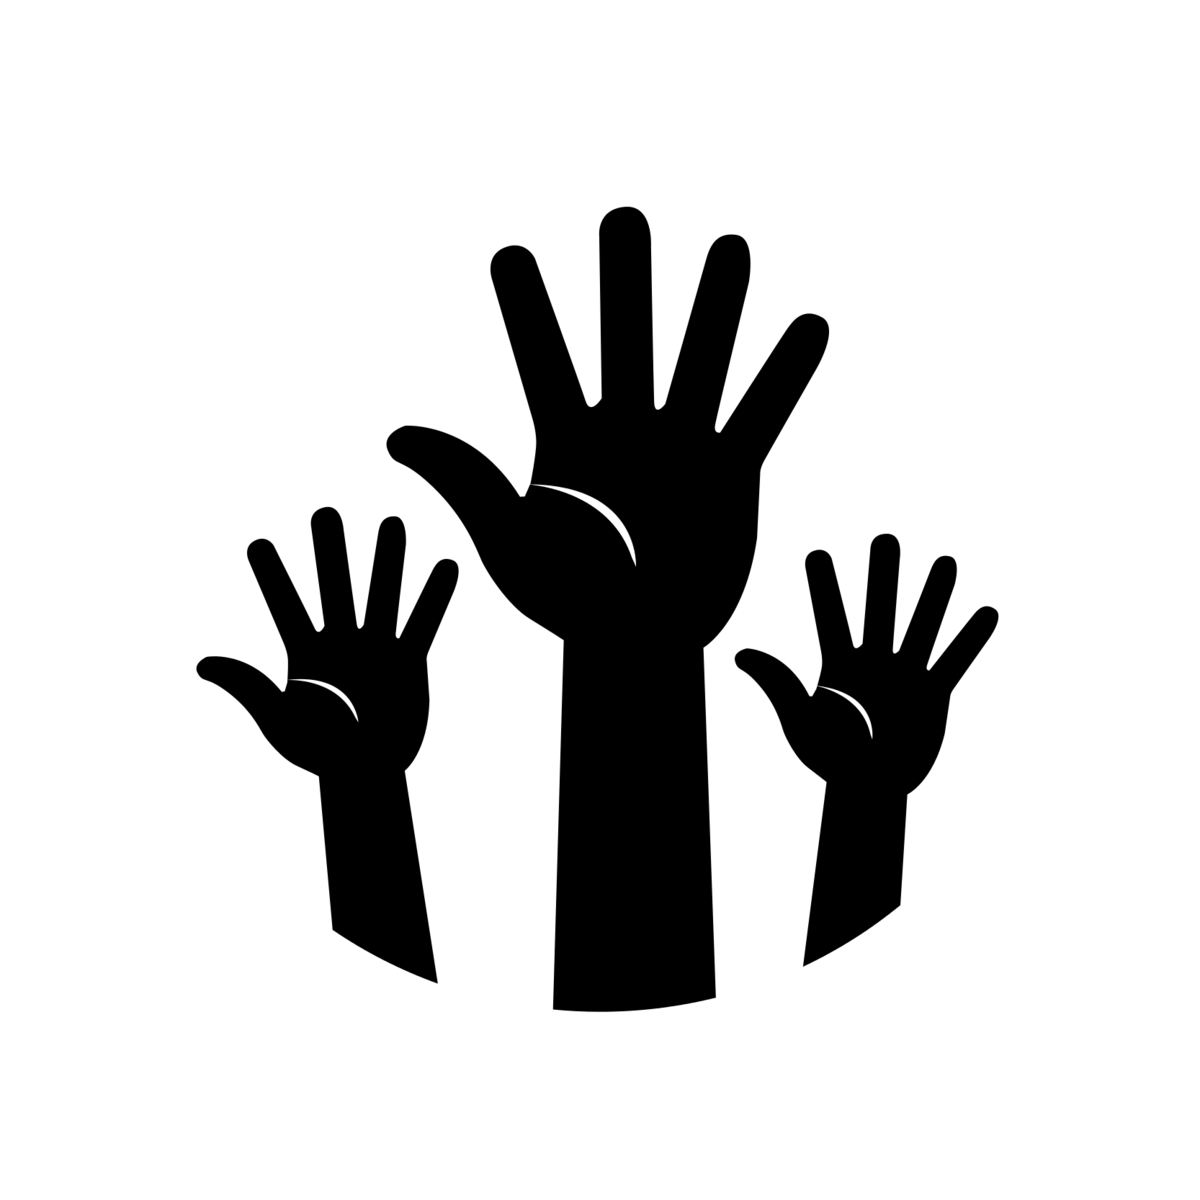
\includegraphics[height=1.5em]{images/hands}}
\newcommand{\transpose}[0]{{\textrm{\tiny{\sf{T}}}}}
\newcommand{\norm}{{\mathcal{N}}}
\newcommand{\cutoff}[0]{\kappa}
\newcommand{\instD}[0]{\dataset}
\newcommand{\insts}[0]{\mathcal{I}}
\newcommand{\inst}[0]{i}
\newcommand{\instI}[1]{i^{(#1)}}

% Iteration specific instance of variable/function/anything
% Introduced in the BO section, but moved up here to make it available within other macros
\newcommand{\iter}[2][\bocount]{{#2}^{(#1)}}

%--------HPO parameter macros-----------

% Parameter Configuration Space
\newcommand{\pcs}[0]{\pmb{\Lambda}}

% ???
\newcommand{\bx}[0]{\conf}

% Parameter Configuration
\newcommand{\conf}[0]{\pmb{\lambda}}

% Final Configuration
\newcommand{\finconf}[0]{\pmb{\hat{\lambda}}}

% Configuration corresponding to a given iteration -- better use \iter!
\newcommand{\confI}[1]{{\conf}^{(#1)}}

% Default Configuration
\newcommand{\defconf}[0]{{\conf}_{\text{def}}}

% Incumbent Configuration
\newcommand{\incumbent}[1][\bocount]{\iter[#1]{\finconf}}

% Optimal Configuration
\newcommand{\optconf}[0]{{\conf}^*}

% Configuration Space
\newcommand{\confs}[0]{\pcs}

%----------------------------------------

%\newcommand{\vlambda}[0]{\bm{\lambda}}
%\newcommand{\vLambda}[0]{\bm{\Lambda}}
\newcommand{\dataset}[0]{\mathcal{D}}
\newcommand{\datasets}[0]{\mathbf{D}}
\newcommand{\loss}[0]{L}
\newcommand{\risk}{\mathcal{R}}
\newcommand{\riske}{\mathcal{R}_{\text{emp}}}
\newcommand{\cost}[0]{c}
\newcommand{\costI}[1]{c^{(#1)}}

% Gaussian Process
\newcommand{\gp}{\mathcal{G}}
% Family of Objective Functions
\newcommand{\objF}{F}

%---------------BO Macros------------------

% BO loop counter
\newcommand{\bocount}{t}
% BO loop counter max, the counter runs from 1 to this value
\newcommand{\bobudget}{T}
% BO loop observation
\newcommand{\obs}[1][\conf]{\cost({#1})}
% BO loop observation space
\newcommand{\obsspace}{\mathcal{Y}}
% BO loop next observation
\newcommand{\bonextobs}{\obs[\iter{\conf}]}
% Acquisition Function, no args
\newcommand{\acq}{u}
% Standard Normal PDF
\newcommand{\pdf}{\phi}
% Standard Normal CDF
\newcommand{\cdf}{\Phi}
% Mean
\newcommand{\mean}{\mu}
% Standard Deviation
\newcommand{\stddev}{\sigma}
% Variance
\newcommand{\variance}{\sigma^2}
% Noise
\newcommand{\noise}{\nu}
% BO loop next selected sample
\newcommand{\bonextsample}{\confI{\bocount}}

% Single hyperparameter
\newcommand{\hyperparam}{\lambda}

% Single hyperparameter within a hyperparameter configuration
\newcommand{\hyperparami}[1][i]{{\hyperparam}_#1}

% Full definition of final configuration
\newcommand{\finconffull}{\incumbent[\bobudget]}

% Dataset
\newcommand{\datasetHPO}{{\dataset}_{HPO}}

% Dataset definition
\newcommand{\datasetHPOdef}{{\langle \bonextsample,\,\bonextobs \rangle}_{\bocount=1}^{\bobudget}}

% Double Display Fraction, forces large displays for everything in numerator and denominator
\newcommand\ddfrac[2]{\frac{\displaystyle #1}{\displaystyle #2}}

% Conditional Probability "Given That" Relation, source:https://tex.stackexchange.com/a/141685/205886
\newcommand\given[1][]{\:#1\vert\:}

% Expectation as a math operator
\DeclareMathOperator*{\E}{\mathbb{E}}

% Citation 
\newcommand{\source}[1]{
    \begin{flushright}
    	Source: \lit{#1}
    \end{flushright}
}
%-------------------------------------------

%Real numbers set
\newcommand{\realnum}{\mathbb{R}}
%Configuration space - do not use
%\newcommand{\configspace}{\Theta}
%Instances - do not use
%\newcommand{\instances}{\mathcal{I}}
%Expected value
\newcommand{\expectation}{\mathbb{E}}
%Kernel
\newcommand{\kernel}{\kappa}
%Constraint function
\newcommand{\constraintf}{c}
%Normal distribution
\newcommand{\normaldist}{\mathcal{N}}

% \renewcommand{\vec}[1]{\mathbf{#1}}
\newcommand{\hist}[0]{\dataset_{\text{Hist}}}
\newcommand{\param}[0]{p}
\newcommand{\algo}[0]{\mathcal{A}}
\newcommand{\algos}[0]{\mathbf{A}}
%\newcommand{\nn}[0]{N}
\newcommand{\feats}[0]{\mathcal{X}_{\text{meta}}}
\newcommand{\feat}[0]{\x_{\text{meta}}}
%\newcommand{\cluster}[0]{\vec{h}}
%\newcommand{\clusters}[0]{\vec{H}}
\newcommand{\perf}[0]{\mathbb{R}}
%\newcommand{\surro}[0]{\mathcal{S}}
\newcommand{\surro}[0]{\hat{\cost}}
\newcommand{\func}[0]{f}
\newcommand{\epm}[0]{\surro}
\newcommand{\portfolio}[0]{\mathbf{P}}
\newcommand{\schedule}[0]{\mathcal{S}}

% Machine Learning
\newcommand{\mdata}[0]{\dataset_{\text{meta}}}
\newcommand{\datasettrain}[0]{\dataset_{\text{train}}}
\newcommand{\datasetval}[0]{\dataset_{\text{val}}}
\newcommand{\datasettest}[0]{\dataset_{\text{test}}}
\newcommand{\x}[0]{\mathbf{x}}
\newcommand{\y}[0]{y}
\newcommand{\xI}[1]{\mathbf{x}^{(#1)}}
\newcommand{\yI}[1]{y^{(#1)}}
\newcommand{\fx}{f(\mathbf{x})}  % f(x), continuous prediction function
\newcommand{\Hspace}{\mathcal{H}} % hypothesis space where f is from
\newcommand{\fh}{\hat{f}}       % f hat, estimated prediction function

% Deep Learning
\newcommand{\weights}[0]{\theta}
\newcommand{\metaweights}[0]{\phi}


% reinforcement learning
\newcommand{\policies}[0]{\mathbf{\Pi}}
\newcommand{\policy}[0]{\pi}
\newcommand{\actionRL}[0]{a}
\newcommand{\stateRL}[0]{s}
\newcommand{\statesRL}[0]{\mathcal{S}}
\newcommand{\rewardRL}[0]{r}
\newcommand{\rewardfuncRL}[0]{\mathcal{R}}

\RestyleAlgo{algoruled}
\DontPrintSemicolon
\LinesNumbered
\SetAlgoVlined
\SetFuncSty{textsc}

\SetKwInOut{Input}{Input}
\SetKwInOut{Output}{Output}
\SetKw{Return}{return}

%\newcommand{\changed}[1]{{\color{red}#1}}

%\newcommand{\citeN}[1]{\citeauthor{#1}~(\citeyear{#1})}

\renewcommand{\vec}[1]{\mathbf{#1}}
\DeclareMathOperator*{\argmin}{arg\,min}
\DeclareMathOperator*{\argmax}{arg\,max}

%\newcommand{\aqme}{\textit{AQME}}
%\newcommand{\aslib}{\textit{ASlib}}
%\newcommand{\llama}{\textit{LLAMA}}
%\newcommand{\satzilla}{\textit{SATzilla}}
%\newcommand{\satzillaY}[1]{\textit{SATzilla'{#1}}}
%\newcommand{\snnap}{\textit{SNNAP}}
%\newcommand{\claspfolioTwo}{\textit{claspfolio~2}}
%\newcommand{\flexfolio}{\textit{FlexFolio}}
%\newcommand{\claspfolioOne}{\textit{claspfolio~1}}
%\newcommand{\isac}{\textit{ISAC}}
%\newcommand{\eisac}{\textit{EISAC}}
%\newcommand{\sss}{\textit{3S}}
%\newcommand{\sunny}{\textit{Sunny}}
%\newcommand{\ssspar}{\textit{3Spar}}
%\newcommand{\cshc}{\textit{CSHC}}
%\newcommand{\cshcpar}{\textit{CSHCpar}}
%\newcommand{\measp}{\textit{ME-ASP}}
%\newcommand{\aspeed}{\textit{aspeed}}
%\newcommand{\autofolio}{\textit{AutoFolio}}
%\newcommand{\cedalion}{\textit{Cedalion}}
\newcommand{\fanova}{\textit{fANOVA}}
\newcommand{\sbs}{\textit{SB}}
\newcommand{\oracle}{\textit{VBS}}

% like approaches
\newcommand{\claspfoliolike}[1]{\texttt{claspfolio-#1-like}}
\newcommand{\satzillalike}[1]{\texttt{SATzilla'#1-like}}
\newcommand{\isaclike}{\texttt{ISAC-like}}
\newcommand{\ssslike}{\texttt{3S-like}}
\newcommand{\measplike}{\texttt{ME-ASP-like}}

\newcommand{\irace}{\textit{I/F-race}}
\newcommand{\gga}{\textit{GGA}}
\newcommand{\smac}{\textit{SMAC}}
\newcommand{\paramils}{\textit{ParamILS}}
\newcommand{\spearmint}{\textit{Spearmint}}
\newcommand{\tpe}{\textit{TPE}}


\usepackage{pifont}
\newcommand{\itarrow}{\mbox{\Pisymbol{pzd}{229}}}
\newcommand{\ithook}{\mbox{\Pisymbol{pzd}{52}}}
\newcommand{\itcross}{\mbox{\Pisymbol{pzd}{56}}}
\newcommand{\ithand}{\mbox{\raisebox{-1pt}{\Pisymbol{pzd}{43}}}}

%\DeclareMathOperator*{\argmax}{arg\,max}

\newcommand{\ie}{{\it{}i.e.\/}}
\newcommand{\eg}{{\it{}e.g.\/}}
\newcommand{\cf}{{\it{}cf.\/}}
\newcommand{\wrt}{\mbox{w.r.t.}}
\newcommand{\vs}{{\it{}vs\/}}
\newcommand{\vsp}{{\it{}vs\/}}
\newcommand{\etc}{{\copyedit{etc.}}}
\newcommand{\etal}{{\it{}et al.\/}}

\newcommand{\pscProc}{{\bf procedure}}
\newcommand{\pscBegin}{{\bf begin}}
\newcommand{\pscEnd}{{\bf end}}
\newcommand{\pscEndIf}{{\bf endif}}
\newcommand{\pscFor}{{\bf for}}
\newcommand{\pscEach}{{\bf each}}
\newcommand{\pscThen}{{\bf then}}
\newcommand{\pscElse}{{\bf else}}
\newcommand{\pscWhile}{{\bf while}}
\newcommand{\pscIf}{{\bf if}}
\newcommand{\pscRepeat}{{\bf repeat}}
\newcommand{\pscUntil}{{\bf until}}
\newcommand{\pscWithProb}{{\bf with probability}}
\newcommand{\pscOtherwise}{{\bf otherwise}}
\newcommand{\pscDo}{{\bf do}}
\newcommand{\pscTo}{{\bf to}}
\newcommand{\pscOr}{{\bf or}}
\newcommand{\pscAnd}{{\bf and}}
\newcommand{\pscNot}{{\bf not}}
\newcommand{\pscFalse}{{\bf false}}
\newcommand{\pscEachElOf}{{\bf each element of}}
\newcommand{\pscReturn}{{\bf return}}

%\newcommand{\param}[1]{{\sl{}#1}}
\newcommand{\var}[1]{{\it{}#1}}
\newcommand{\cond}[1]{{\sf{}#1}}
%\newcommand{\state}[1]{{\sf{}#1}}
%\newcommand{\func}[1]{{\sl{}#1}}
\newcommand{\set}[1]{{\Bbb #1}}
%\newcommand{\inst}[1]{{\tt{}#1}}
\newcommand{\myurl}[1]{{\small\sf #1}}

\newcommand{\Nats}{{\Bbb N}}
\newcommand{\Reals}{{\Bbb R}}
\newcommand{\extset}[2]{\{#1 \; | \; #2\}}

\newcommand{\vbar}{$\,\;|$\hspace*{-1em}\raisebox{-0.3mm}{$\,\;\;|$}}
\newcommand{\vendbar}{\raisebox{+0.4mm}{$\,\;|$}}
\newcommand{\vend}{$\,\:\lfloor$}


\newcommand{\goleft}[2][.7]{\parbox[t]{#1\linewidth}{\strut\raggedright #2\strut}}
\newcommand{\rightimage}[2][.3]{\mbox{}\hfill\raisebox{1em-\height}[0pt][0pt]{\includegraphics[width=#1\linewidth]{#2}}\vspace*{-\baselineskip}}






\title{AutoML: Bayesian Optimization for HPO}
\subtitle{Surrogate Models}
\author[Marius Lindauer]{Bernd Bischl \and \underline{Frank Hutter} \and Lars Kotthoff\newline \and Marius Lindauer \and Joaquin Vanschoren}
\institute{}
\date{}
    
    
    
\begin{document}
\maketitle

%-----------------------------------------------------------------------
\myframetop{Desiderata for Surrogate Models in Bayesian Optimization}{

    \begin{columns}[T] % align columns
    \begin{column}{.48\textwidth}
    \only<1-2>{
        \begin{block}{In all cases}
        \begin{itemize}
        	\item Regression model with uncertainty estimates
        	\item Accurate predictions
        \end{itemize}
        \end{block}
    }
    \only<2-2>{
        \begin{block}{Depending on the application}
        \begin{itemize}
        	\item Is cheap to train
        	\item Scales well in the number of data points
        	\item Scales well in the number of dimensions
        	\item Can handle different types of inputs (categorical and continuous)
        \end{itemize}
        \end{block}
    }
    \end{column}%
    
    \hfill%
    
    \begin{column}{.48\textwidth}
    \bigskip
    \bigskip
    %\only<1-1>{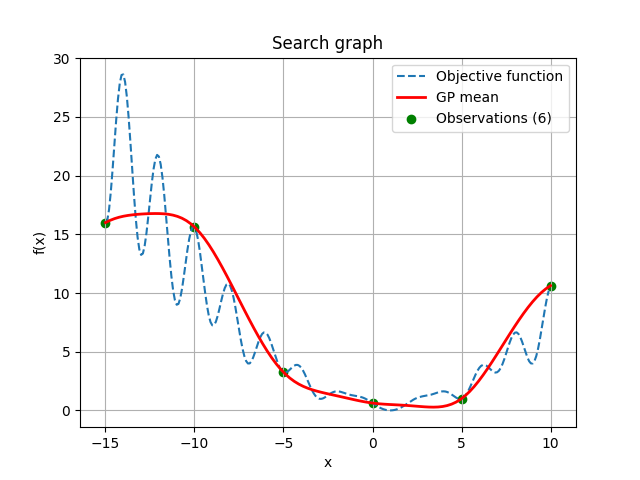
\includegraphics[width=1.\textwidth]{images/bo_loop_overview/03_mean.png}}
    %\only<2-6>{
    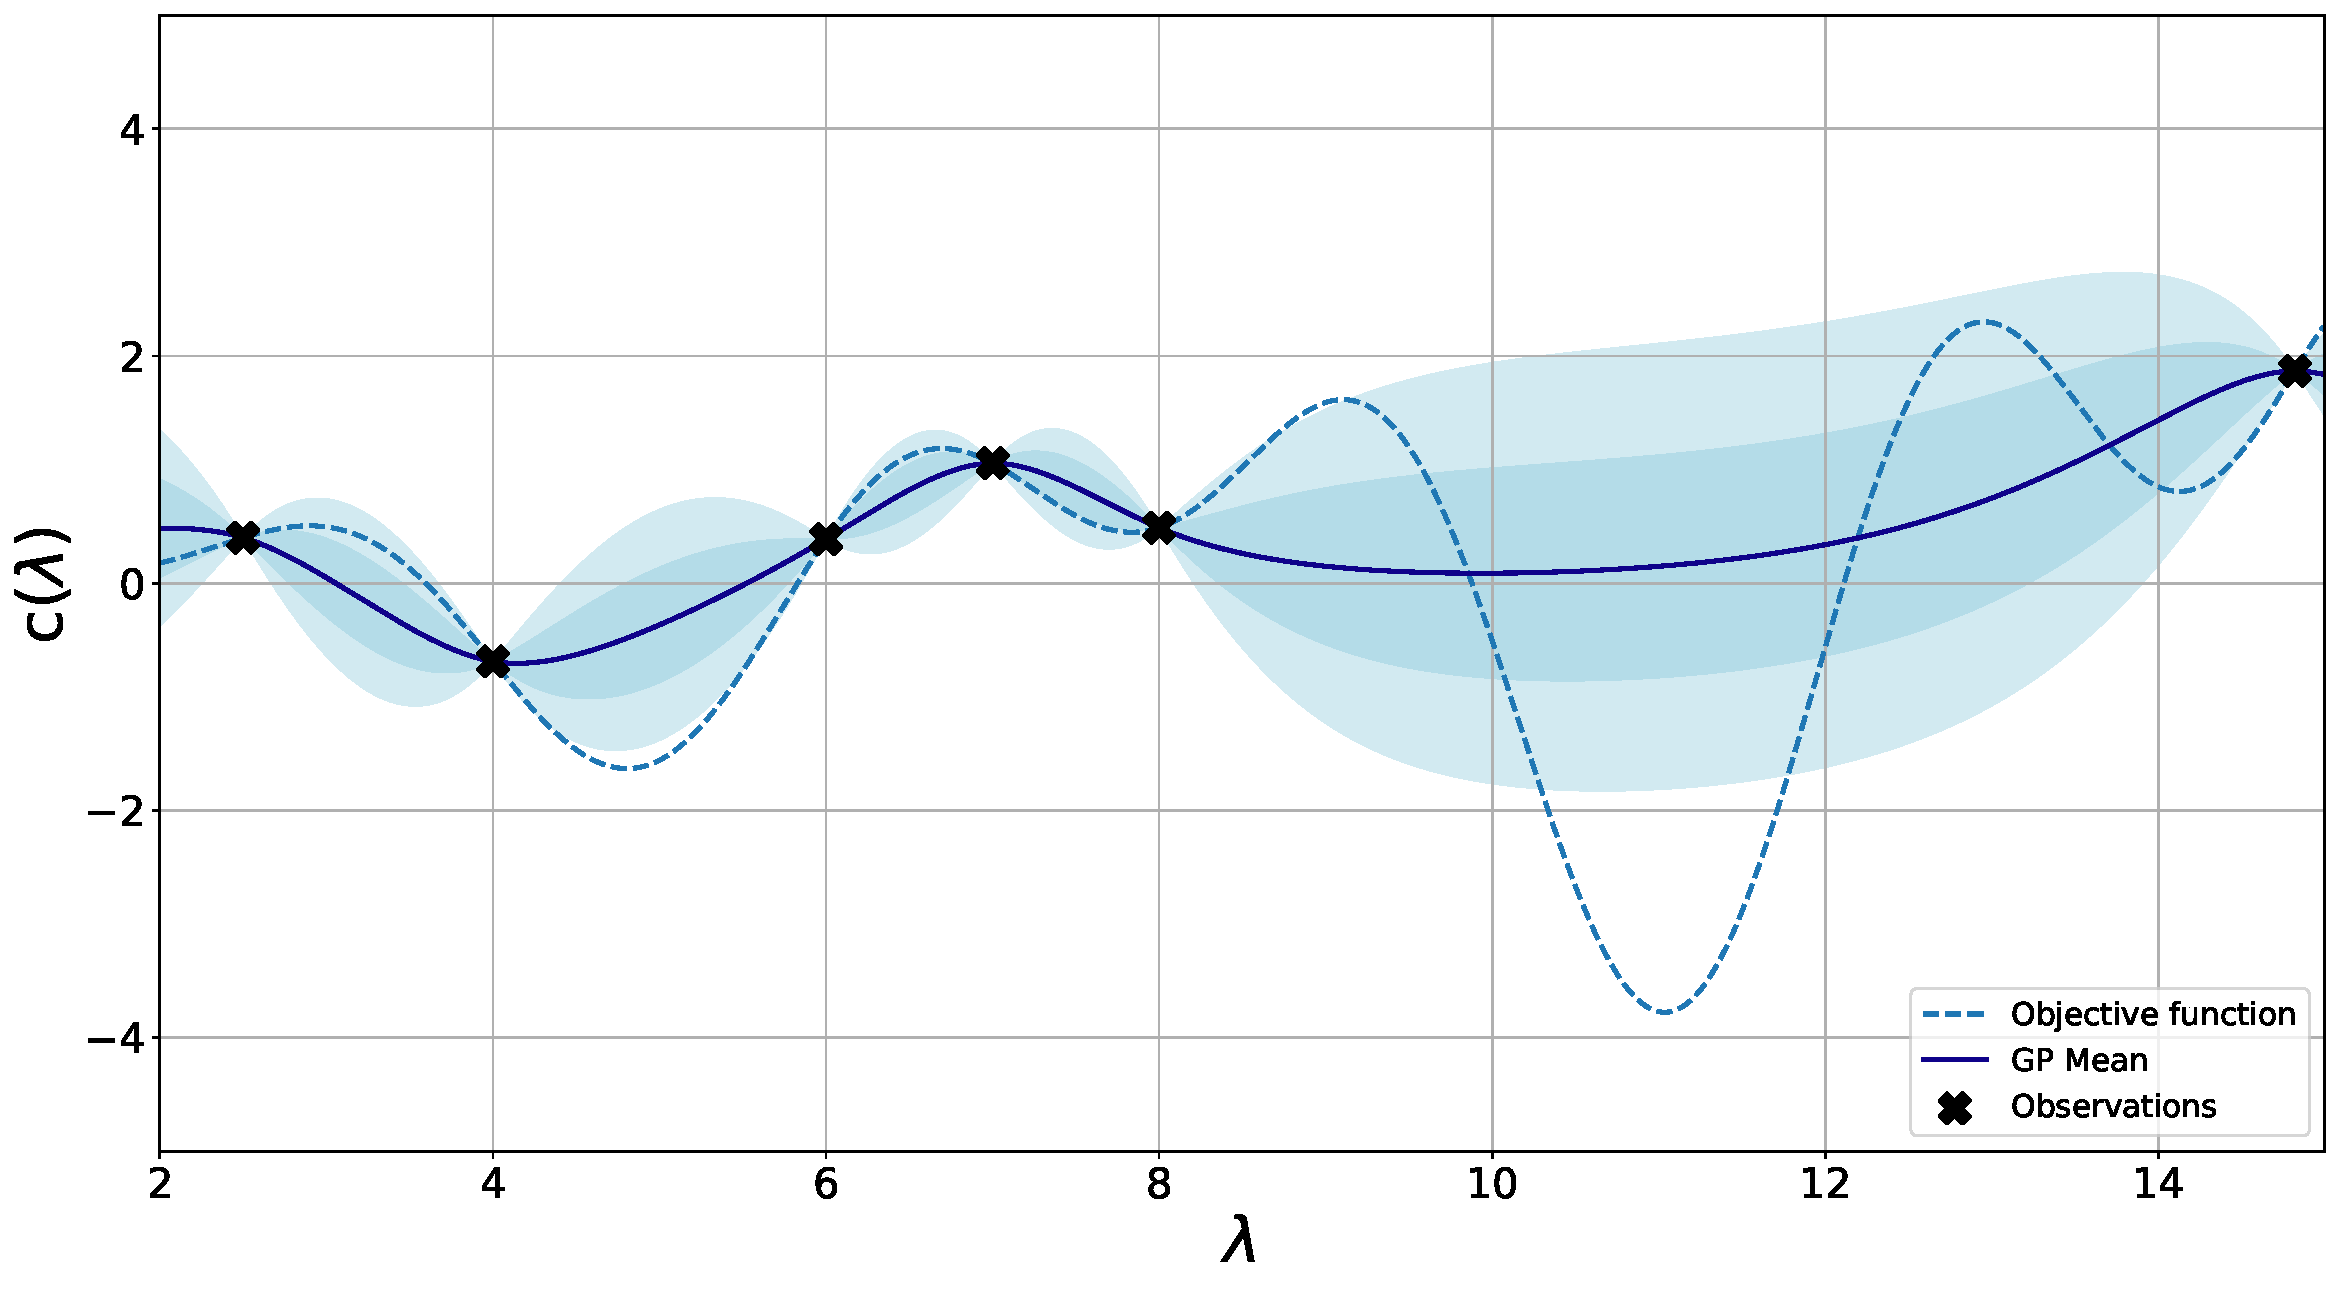
\includegraphics[width=\textwidth]{images/bo_loop_overview/Uncertainty.pdf}
    %}
    
    \end{column}%
    \end{columns}
}
%-----------------------------------------------------------------------

%-----------------------------------------------------------------------
%-----------------------------------------------------------------------
\begin{frame}[c]{Overview of the Surrogate Models We'll Discuss}

%\begin{columns}[T] % align columns
%\begin{column}{.38\textwidth}
%\begin{minipage}[c][.6\textheight][c]{\linewidth}
\begin{itemize}
	\item Gaussian Processes \note[item]{(quite common)}
	\item Random Forests \note[item]{(our default choice)}
	\item Bayesian Neural Networks \note[item]{(recent trend)}

\end{itemize}
%\end{minipage}
%\end{column}%

%\hfill%
%\begin{column}{.58\textwidth}
%
%\begin{columns}[T] % align columns
%\begin{column}{.48\textwidth}
%    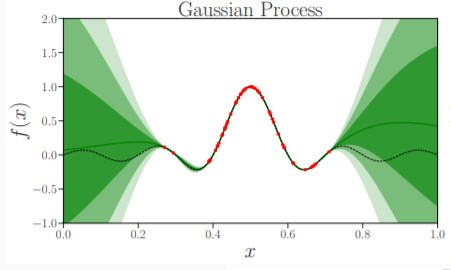
\includegraphics[width=1.\textwidth]{images/surrogate_models/uncertainty_gp.jpg}
%\end{column}%
%
%\hfill%
%
%\begin{column}{.48\textwidth}
%    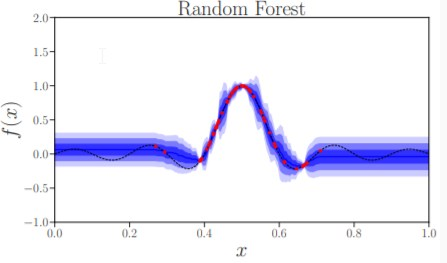
\includegraphics[width=1.\textwidth]{images/surrogate_models/uncertainty_forest.jpg}
%\end{column}%
%\end{columns}
%
%\vspace*{\fill}
%\begin{center}
%  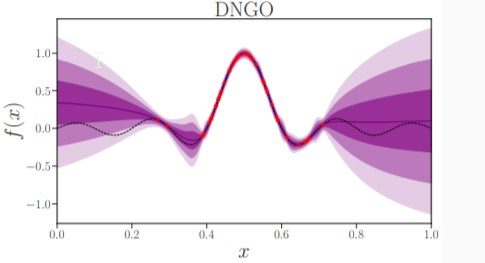
\includegraphics[width=.6\textwidth]{images/surrogate_models/uncertainty_dngo.jpg}
%  
%\end{center}
%\vspace*{\fill}
%
%\end{column}%
%\end{columns}
%
%\hspace{5.5cm}\footnotesize{Image source: \lit{\href{}{A. Klein: Introduction Automated Machine Learning}}}


\end{frame}
%-----------------------------------------------------------------------
\begin{frame}[c]{Gaussian Processes (GPs): Reminder of Pros and Cons}

\begin{columns}[T] % align columns
\begin{column}{.48\textwidth}

    \begin{block}{Advantages}
    \begin{itemize}
    	\item Smooth and reliable uncertainty estimates 
		\item Strong sample efficiency
    	\item We can encode expert knowledge about the design space in the kernel 
    \end{itemize}
    \end{block}
\bigskip
\pause
\hspace*{0.5cm}These advantages make GPs the\\
\hspace*{0.5cm}\alert{most commonly-used model\\
\hspace*{0.5cm}in Bayesian optimization}

\end{column}%

\hfill%
\pause

\begin{column}{.48\textwidth}
    \begin{block}{Disadvantages}
    \begin{itemize}
    	\item Performance can be quite sensitive to the choice of kernel
    	\note[item]{(if we don't optimize small-dimensional, continuous functions)}
    	\item Cost scales cubically with the number of observations 
    	\item Weak performance for high dimensionality
    	\note[item]{(because of inverting the kernel)}
    	\item Not easily applicable in discrete or conditional spaces 
    	\item Sensitive to its own hyperparameters
    \end{itemize}
\end{block}

\end{column}
\end{columns}

\note[item]{
	\begin{itemize}
		 \item e.g., special kernels for categorical hyperparameters and\\ conditional dependencies
	\end{itemize}
}
	
\note[item]{
    \begin{itemize}
    	\item to address this issue, there are sparse GPs\\ \lit{Snelson and Ghahramani. 2005}
    \end{itemize}
}

\end{frame}
%-----------------------------------------------------------------------

%-----------------------------------------------------------------------
%-----------------------------------------------------------------------
%\begin{frame}[c]{Gaussian Processes - reminder}
%
%\begin{itemize}
%    \item<1-3> The prior is a GP with constant mean and variance; draws are jointly Gaussian
%    \item<2-3> The kernel (covariance) function $K$ tells us how correlated the function values at two points are
%    \item<3-3> The posterior is also a GP, with predictive distribution:
 %   \begin{equation*}
 %        P(\func_{\bocount+1} \vert \dataset_{1:\bocount}, \conf_{\bocount+1}) =  \mathcal{N}(\mean_{\bocount}(\conf_{\bocount+1}), \variance_{\bocount}(\conf_{\bocount+1}))
 %   \end{equation*}
 %   \begin{equation*}
 %       \mean_{\bocount}(\conf_{\bocount+1}) = \bm{k}^{T} \bm{K}^{-1} \bm{\func_{1:\bocount}}
 %   \end{equation*}
 %   \begin{equation*}
 %       \variance_{\bocount}(\conf_{\bocount+1}) = k(\conf_{\bocount+1}, \conf_{\bocount+1}) - \bm{k}^{T} \bm{K}^{-1} \bm{k}
 %   \end{equation*}
%\end{itemize}
%
%\note[item]{for the review of GPs - Rasmussen and Williams}
%
%\end{frame}
%-----------------------------------------------------------------------
 
% %-----------------------------------------------------------------------
% %-----------------------------------------------------------------------
% \begin{frame}[c]{Surrogate Models: GPs - kernel hyperparameters}

% \begin{itemize}
%     \item After choosing the kernel, we must also manage the hyperparameters that govern its behaviour, as well as that of the mean function.  \fhpause
%     \item For our problems of interest, typically we have $D + 3$ GPs hyperparameters:  
%     \begin{itemize}
%         \item $D$ length scales $\theta_{1:D}$, 
%         \item the covariance amplitude $\theta_{0}$, 
%         \item the observation noise $\noise$, 
%         \item a constant mean $\mean$. 
%     \end{itemize}
% \end{itemize}

% \end{frame}
% %-----------------------------------------------------------------------


%-----------------------------------------------------------------------
%-----------------------------------------------------------------------
\begin{frame}[c]{Gaussian Processes (GPs): Kernel Hyperparameters}

\begin{columns}[T] % align columns
\begin{column}{.6\textwidth}
\begin{itemize}
    \item We could optimize GP hyperparameters (maximum likelihood, MLE, or maximum a posteriori, MAP)


    \item<+-> But \alert{sampling} GP  hyperparameters from the posterior distribution performs better; e.g., via \alert{Markov-Chain Monte-Carlo (MCMC)}


    \item<+-> \alert{Marginalize} over GP hyperparameters $\theta$ and compute an \alert{integrated acquisition function}:
        \begin{equation*}
        \begin{aligned}
            \Bar{\acq}(\conf) = \int \acq (\conf, \surro_\theta)p(\theta)d\theta
        \end{aligned}
        \end{equation*}

 
    \item<+-> Downside: computational expense
    \myit{
        \item MCMC is computationally expensive
        \item Acquisition function now has to be calculated for each sample
    }
\end{itemize}
\end{column}
%
\begin{column}{.4\textwidth}
\only<2->{
    \centering
    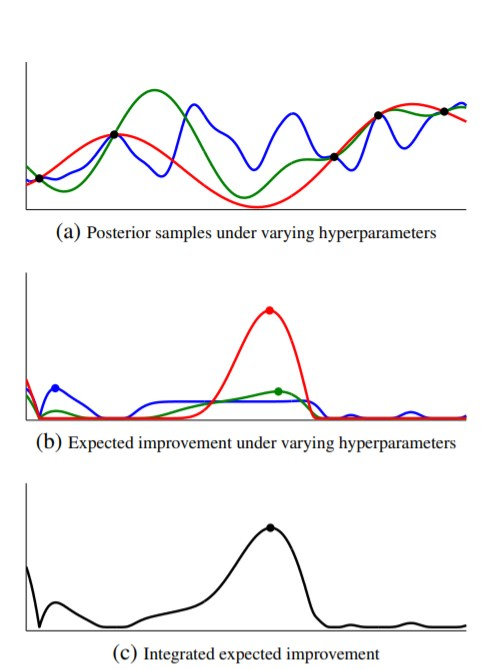
\includegraphics[width=0.7\textwidth]{images/surrogate_models/kernel_hp_mcmc.jpg}
    
    \footnotesize{Image source: \lit{\href{https://arxiv.org/pdf/1206.2944.pdf}{Snoek et al. 2012}}}
}


   
\end{column}

\end{columns}

\end{frame}
%-----------------------------------------------------------------------
\begin{frame}[c]{Random Forests (RFs): Reminder \& How To Compute Uncertainties}

\centering
    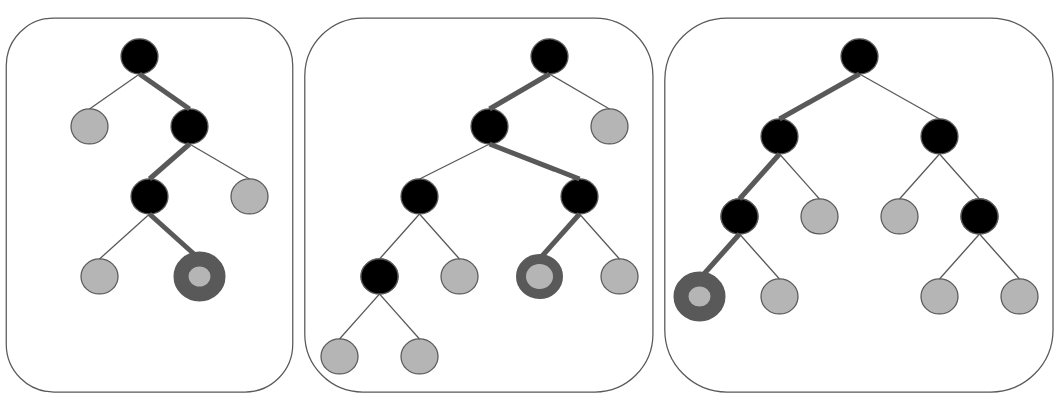
\includegraphics[width=0.5\textwidth]{images/surrogate_models/random_forest_pic}

\begin{columns}[T] % align columns
\begin{column}{.48\textwidth}

\begin{block}{RF Training}
\begin{itemize}
	\item Fit a set of \alert{randomized} regression trees
	\item Randomization via bootstrapping \& random selection of split variables / split points
	\item Each tree yields a possible explanation for the observations
\end{itemize}
\end{block}
\end{column}

\pause
\hfill

\begin{column}{.48\textwidth}
    \begin{block}{RF Prediction}
    \begin{itemize}
    	\item Predict with each tree
    	\item Aggregate predictions (e.g., average)
    	\item Uncertainty estimate:\\ \alert{empirical variance across tree predictions}
    \end{itemize}
    \end{block}
\end{column}
\end{columns}

\end{frame}
%-----------------------------------------------------------------------
\begin{frame}[c]{Random Forests (RFs): Impact of Basic Model Choices}
\vspace{-25pt}

\begin{columns}
\column{0.5\textwidth}

\begin{figure}[h]
\captionsetup[subfigure]{position=top}
\centering

\renewcommand{\thesubfigure}{a}
\subfloat[][no bootstrapping, \\ no random splits]{
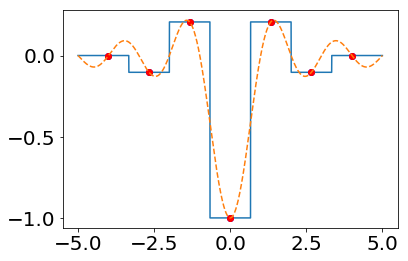
\includegraphics[width=0.55\textwidth, clip]{images/surrogate_models/rf_noboot_middle_split.png}

}
\qquad
\renewcommand{\thesubfigure}{b}
\subfloat[][with bootstrapping, \\ no random splits]{
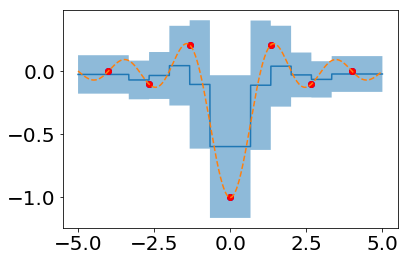
\includegraphics[width=0.55\textwidth, clip]{images/surrogate_models/rf_boot_middle_split.png}
}
\end{figure}

\column{0.5\textwidth}
\begin{figure}[h]
\captionsetup[subfigure]{position=top}
\centering

\pause
\renewcommand{\thesubfigure}{c}
\subfloat[][no bootstrapping, \\ with random splits]{
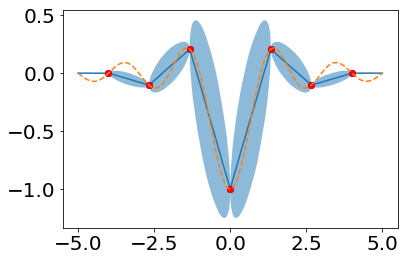
\includegraphics[width=0.55\textwidth, clip]{images/surrogate_models/rf_noboot_rand_split.png}

}
\qquad
\renewcommand{\thesubfigure}{d}
\subfloat[][with bootstrapping, \\ with random splits]{
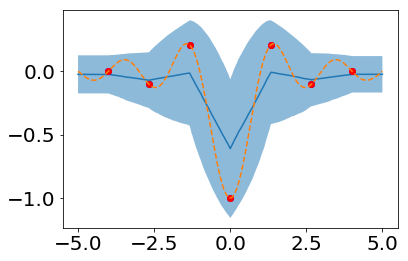
\includegraphics[width=0.55\textwidth, clip]{images/surrogate_models/rf_boot_rand_split.png}
}

\end{figure}
\end{columns}

\end{frame}
%-----------------------------------------------------------------------
\begin{frame}[c]{Random Forests (RFs): Overview of Pros and Cons}

\begin{columns}[T] % align columns
\begin{column}{.48\textwidth}

    \begin{block}{Advantages}
    \begin{itemize}
        \item Cheap to train 
        \item Scales well with \#observations $n$: 
        \begin{itemize}
        	\item Fitting: $O(n \log n)$ 
        	\item Prediction: $O(\log n)$
        \end{itemize}
        \item Scales well with \#dimensions
        \item Training can be parallelized 
        \item Can easily handle conditional, categorical, continuous and discrete spaces 
        \item Quite robust against its own hyperparameters
    \end{itemize}
    \end{block}
\end{column}%

\hfill%
\pause

\begin{column}{.48\textwidth}
    \begin{block}{Disadvantages}
    \begin{itemize}
        \item Poor uncertainty estimates 
        \item Poor extrapolation (constant) 
    	\item Priors cannot be incorporated easily 
    \end{itemize}
    \end{block}

\pause
\bigskip
\bigskip
\hspace*{0.5cm}These qualities make RFs a \alert{robust} \\
\hspace*{0.5cm}\alert{option} for Bayesian optimization in \\ \hspace*{0.5cm}\alert{high dimensions}, for \alert{categorical spaces},\\
\hspace*{0.5cm}or when function evaluations are quite fast

\end{column}
\end{columns}

\end{frame}
%-----------------------------------------------------------------------
\begin{frame}[c]{Bayesian Neural Networks: Overview}

\begin{itemize}
    \item Neural networks are more flexible \& scalable than Gaussian processes 
    \item But for use in Bayesian optimization, neural networks need to be made probabilistic
    
\pause
    \item Bayesian deep learning aims to deal with all sources of uncertainty \pause
    \begin{itemize}
        \item E.g., we don't have a single weight vector anymore, but a distribution over weights
    \end{itemize}

\centering
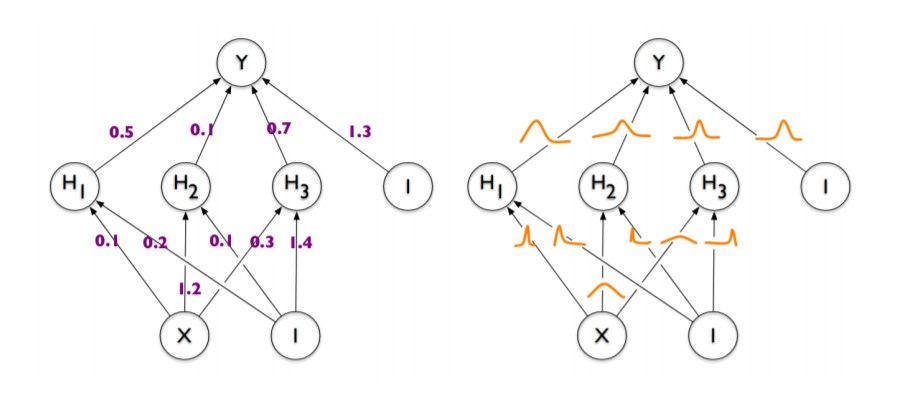
\includegraphics[width=0.6\textwidth]{images/surrogate_models/bnn.jpg}

\footnotesize{Image source: \lit{\href{http://proceedings.mlr.press/v37/blundell15.pdf}{Blundell et al. 2015}}}

\end{itemize}



\end{frame}
%-----------------------------------------------------------------------
%\begin{frame}[c]{Surrogate Models: Bayesian Neural Networks - Idea}
%
%\begin{itemize}
%    \item Extend regression NNs to model uncertainty
%    \item Deal with all sources of parameter uncertainty
%    \item If possible, one would also deal with uncertainty about the network architecture
%     \begin{itemize}
%        \item For every architecture, one would still want to be Bayesian about its weights... 
%        \item Nobody is really Bayesian about architectures these days 
%        \item This has been too expensive; but that may change with efficient gradient-based architecture search methods...
%    \end{itemize}
%\end{itemize}
%
%\end{frame}

%-----------------------------------------------------------------------

\begin{frame}[c]{Simplest Way of Incorporating Uncertainty in Neural Networks: DNGO}


\begin{itemize}
    \item Fit a standard regression neural network to the data (with a linear output layer)
    \item Use the representation in the last hidden layer as \alert{basis functions $\phi(x)$} of the input $x$ 
    \item \alert{Use Bayesian linear regression with these basis functions} \pause
    \begin{itemize}
        \item The last layer is linear in its parameters $\theta$  
        \item Therefore, the Bayesian linear regression formulas work directly 
        \item Feasible in closed form, in time $O(N d^3)$, where $N$ is the number of data points\\ and $d$ is the number of hidden units in the last layer 
    \end{itemize}
    \item Not fully Bayesian yet, but already allows scalable Bayesian optimization \lit{\href{https://arxiv.org/pdf/1502.05700.pdf}{Snoek et al. 2015}}

\end{itemize}

%\vspace{1cm}
%\hspace{12cm}
%\lit{\href{https://arxiv.org/pdf/1502.05700.pdf}{Snoek et al. 2015}}

\end{frame}


%-----------------------------------------------------------------------

\begin{frame}[c]{Bayesian Optimization with BNNs: Overview of Existing Approaches}

\begin{itemize}
	    \item  Scalable Bayesian Optimization Using Deep Neural Networks (DNGO) \lit{\href{https://arxiv.org/pdf/1502.05700.pdf}{Snoek et al. 2015}}
	    \item  Bayesian Optimization with Robust Bayesian Neural Networks \lit{\href{https://papers.nips.cc/paper/6117-bayesian-optimization-with-robust-bayesian-neural-networks.pdf}{Springenberg et al. 2016}}
	    \item  Parallel and Distributed Thompson Sampling for Large-scale Accelerated Exploration of Chemical Space \lit{\href{https://arxiv.org/pdf/1706.01825.pdf}{Hern\'andez-Lobato et al. 2017}}
\bigskip

\pause
        \item  Hyperparameter Optimization with Factorized Multilayer Perceptrons \lit{\href{https://www.ismll.uni-hildesheim.de/pub/pdfs/schilling2015-ecml.pdf}{Schilling et al. 2015}}
        \item  Scalable Hyperparameter Transfer Learning \lit{\href{https://papers.nips.cc/paper/2018/file/14c879f3f5d8ed93a09f6090d77c2cc3-Paper.pdf}{Perrone et al. 2018}}


\end{itemize}

\end{frame}
%-----------------------------------------------------------------------
\begin{frame}[c]{Bayesian Neural Networks (BNNs): Overview of Pros and Cons}

\begin{columns}[T] % align columns
\begin{column}{.48\textwidth}

    \begin{block}{Advantages}
    \begin{itemize}
        \item Scales linearly with \#observations 
        \item Can obtain nice and smooth uncertainty estimates 
        \item Flexibility: handling of categorical, continuous and discrete spaces
    \end{itemize}
    \end{block}

\onslide<3->{
\bigskip
\bigskip
\hspace*{0.5cm}These qualities make BNNs an \\
\hspace*{0.5cm}\alert{ever-more promising alternative}
%\hspace*{0.5cm}Needed: robust auto-tuned(?) implementation
}
\end{column}%

\hfill%

\begin{column}{.48\textwidth}
\onslide<2->{
    \begin{block}{Disadvantages}
    \begin{itemize}
    	\item Usually needs more data than Gaussian processes
    	\item Uncertainty estimates often worse than for Gaussian processes 
        \item Many meta-design decisions 
    	\item No robust off-the-shelf implementation 
    \end{itemize}
    \end{block}
}
\end{column}
\end{columns}

\end{frame}
%-----------------------------------------------------------------------
\begin{frame}[c]{Bayesian Neural Networks (BNNs): Further Reading}

There is a lot more work on BNNs that hasn't been applied to Bayesian optimization yet:
\begin{itemize}
%        \item \lit{\href{https://www.cs.utoronto.ca/~radford/bnn.book.html}{Neal 1995}} Bayesian Learning for Neural Networks
%        \item \lit{\href{https://www.microsoft.com/en-us/research/uploads/prod/2006/01/Bishop-Pattern-Recognition-and-Machine-Learning-2006.pdf}{Bishop 2006}} Pattern Recognition and Machine Learning
        \item Ensembles obtained simply by running SGD several times \lit{\href{https://arxiv.org/pdf/1612.01474.pdf}{Lakshminarayanan et al. 2016}}
        %: Simple and Scalable Predictive Uncertainty Estimation using Deep Ensembles
        \item Dropout \lit{\href{https://arxiv.org/pdf/1506.02142.pdf}{Gal and Ghahramani. 2015}} 
        %Dropout as a Bayesian Approximation:
        %Representing Model Uncertainty in Deep Learning
        \item Monte Carlo Batch Normalization \lit{\href{https://arxiv.org/pdf/1802.06455.pdf}{Teye et al. 2018}} %Bayesian Uncertainty Estimation for Batch Normalized Deep Networks
        \item Snapshot Ensembles \lit{\href{https://arxiv.org/pdf/1704.00109.pdf}{Gao Huang et al. 2017}} 
        %Snapshot Ensembles: Train 1, get M for free
\end{itemize}


\end{frame}
%-----------------------------------------------------------------------
\begin{frame}[c]{Questions to Answer for Yourself / Discuss with Friends}

\begin{itemize}
    %GP
%    \item \alert{Repetition.} What are the most important hyperparameters of a GP that you would want to optimize for Bayesian Optimization? 
    %RF
    \item \alert{Discussion.} For which optimization problems would you rather use a RF than a GP? When would you use a BNN?
\medskip
%BNN
%    \item \alert{Discussion.} Can a BNN be trained with standard MCMC in theory and in practice?
    %DNGO
    \item \alert{Discussion.} Why can DNGO's Bayesian Linear Regression approach only be applied to the last layer of a Deep Neural Network, not to all layers?
\medskip    
    \item \alert{Open Question.} All of the surrogate models we saw have pros and cons. Would it be possible to select the best model (and its hyperparameters) dependent on the data at hand, and could this be done effectively? (This is a possible research project.)

\end{itemize}
\end{frame}
\end{document}